\documentclass{beamer}
\usetheme{Boadilla}
% \setbeameroption{show notes}

\usepackage[brazil]{babel}
\usepackage[utf-8]{inputenc}
\usepackage{cfr-lm}

\usepackage{lipsum}

\usepackage{tikz}
    \usetikzlibrary{arrows.meta}

\tikzset{
  invisible/.style={opacity=0},
  transparent/.style={opacity=0.1},
  visible on/.style={alt={#1{}{invisible}}},
  uncover/.style={alt={#1{}{transparent}}},
  alt/.code args={<#1>#2#3}{%
    \alt<#1>{\pgfkeysalso{#2}}{\pgfkeysalso{#3}} % \pgfkeysalso doesn't change the path
  },
}

% \tikzset{edge/.append style={thick, -{stealth},}}


\usetikzlibrary{calc}

\newcommand*{\GridSize}{2}

\newcommand*{\ColorCells}[1]{% #1 = list of x/y/color
  \foreach \x/\y/\color in {#1} {
    \node [fill=\color, draw=none, thick, minimum size=1cm] 
      at (\x-.5,\GridSize+0.5-\y) {};
    }%
}%

\newcommand*{\ColorCellsCustomSize}[2]{% #1 = list of x/y/color
  \foreach \x/\y/\color in {#1} {
    \node [fill=\color, draw=none, thick, minimum size=1cm] 
      at (\x-.5,#2+0.5-\y) {};
    \draw (\x, #2-\y) -- (\x - 1, #2-\y) -- (\x - 1, #2-\y+1) -- (\x, #2-\y+1) -- (\x, #2-\y);
    }%
}%

\newcommand{\term}[2]{
    \begin{tikzpicture}[scale=#1, every node/.style={transform shape, rectangle}]
        \begin{scope}[thick,local bounding box=name]
            \ColorCells{#2}
            \draw (0, 0) grid (\GridSize, \GridSize);
        \end{scope}
    \end{tikzpicture}
}

\newcommand*{\TermScale}{0.5}

\newcommand*{\vl}{
    \begin{tikzpicture}[scale=\TermScale, every node/.style={transform shape}]
        \begin{scope}[thick,local bounding box=name]
            % \ColorCells{#2}
            \draw (0, 0) -- (0, \GridSize);
        \end{scope}
    \end{tikzpicture}
}

\newcommand*{\constant}[1]{
    \begin{tikzpicture}[scale=\TermScale * \GridSize / (\GridSize + 1), every node/.style={transform shape}]
        \begin{scope}[rectangle, thick,local bounding box=name]
            \draw[opacity=0] (0, 0) grid (\GridSize + 1, \GridSize + 1);
            \draw[shift={(0.5,0.5)}] (0,0) -- (\GridSize, 0) -- (\GridSize, \GridSize) -- (0, \GridSize) -- (0,0);
            \ColorCellsCustomSize{#1}{\GridSize + 1}
        \end{scope}
    \end{tikzpicture}
}

\newcommand*{\BBBB}{\term{\TermScale}{1/1/black, 1/2/black, 2/1/black, 2/2/black}}
\newcommand*{\BBBW}{\term{\TermScale}{1/1/black, 1/2/black, 2/1/black, 2/2/white}}
\newcommand*{\BBWB}{\term{\TermScale}{1/1/black, 1/2/black, 2/1/white, 2/2/black}}
\newcommand*{\BBWW}{\term{\TermScale}{1/1/black, 1/2/black, 2/1/white, 2/2/white}}
\newcommand*{\BWBB}{\term{\TermScale}{1/1/white, 1/2/black, 2/1/black, 2/2/black}}
\newcommand*{\BWBW}{\term{\TermScale}{1/1/white, 1/2/black, 2/1/black, 2/2/white}}
\newcommand*{\BWWB}{\term{\TermScale}{1/1/white, 1/2/black, 2/1/white, 2/2/black}}
\newcommand*{\BWWW}{\term{\TermScale}{1/1/white, 1/2/black, 2/1/white, 2/2/white}}
\newcommand*{\WBBB}{\term{\TermScale}{1/1/black, 1/2/white, 2/1/black, 2/2/black}}
\newcommand*{\WBBW}{\term{\TermScale}{1/1/black, 1/2/white, 2/1/black, 2/2/white}}
\newcommand*{\WBWB}{\term{\TermScale}{1/1/black, 1/2/white, 2/1/white, 2/2/black}}
\newcommand*{\WBWW}{\term{\TermScale}{1/1/black, 1/2/white, 2/1/white, 2/2/white}}
\newcommand*{\WWBB}{\term{\TermScale}{1/1/white, 1/2/white, 2/1/black, 2/2/black}}
\newcommand*{\WWBW}{\term{\TermScale}{1/1/white, 1/2/white, 2/1/black, 2/2/white}}
\newcommand*{\WWWB}{\term{\TermScale}{1/1/white, 1/2/white, 2/1/white, 2/2/black}}
\newcommand*{\WWWW}{\term{\TermScale}{1/1/white, 1/2/white, 2/1/white, 2/2/white}}

\newcommand*{\allTerms}{\BBWW \WWBB \vl \WBWB \WWBW \WWWB}

% Switch implementation
\usepackage{xifthen}
\newcommand{\ifequals}[3]{\ifthenelse{\equal{#1}{#2}}{#3}{}}
\newcommand{\case}[2]{#1 #2} % Dummy, so \renewcommand has something to overwrite...
\newenvironment{switch}[1]{\renewcommand{\case}{\ifequals{#1}}}{}

\newcommand*{\Term}[1]{%
\begin{switch}{#1}  
    \case{1}{\BBWW}%
    \case{2}{\WWBB}%
    \case{3}{\WBWB}%
    \case{4}{\WWBW}%
    \case{5}{\WWWB}%
\end{switch}
}

\newcommand*{\const}[1]{%
\begin{switch}{#1}  
    \case{1}{\constant{1/3/black}}%
    \case{2}{\constant{1/1/black}}%
    \case{3}{\constant{3/1/black}}%
    \case{4}{\constant{3/3/black}}%
    \case{5}{\constant{1/3/white}}%
    \case{6}{\constant{1/1/white}}%
    \case{7}{\constant{3/1/white}}%
    \case{8}{\constant{3/3/white}}%
\end{switch}
}

\newcommand*{\allConstants}{
    \constant{1/3/black}%
    \constant{1/1/black}%
    \constant{3/1/black}%
    \constant{3/3/black}%
    \constant{1/3/white}%
    \constant{1/1/white}%
    \constant{3/1/white}%
    \constant{3/3/white}%
}

\title[AM Algébrico]{Aprendizagem de Máquina Algébrico}
\subtitle{PO-240: Tópicos em Inteligência Artifical}
\institute{ITA}
% \author[Caio \& Fábio \& Johnnie]
\author[Caio Costa]
{%
  \texorpdfstring{
    \begin{columns}%[onlytextwidth]
      \column{.30\linewidth}
      \centering
      Caio Costa\\
      \href{mailto:caio.costa@ga.ita.br}{caio.costa@ga.ita.br}
    \end{columns}
    }{Caio Costa}
}
% {%
%   \texorpdfstring{
%     \begin{columns}%[onlytextwidth]
%       \column{.30\linewidth}
%       \centering
%       Caio Costa\\
%       \href{mailto:caio.costa@ga.ita.br}{caio.costa@ga.ita.br}
%       \column{.30\linewidth}
%       \centering
%       Fábio Alan\\
%       \href{mailto:fabio.alan@ga.ita.br}{fabio.alan@ga.ita.br}
%       \column{.30\linewidth}
%       \centering
%       Johnnie Bastista\\
%       \href{mailto:johnnie@ita.br}{johnnie@ita.br}
%     \end{columns}
%   }
%   {Caio \& Fábio \& Johnnie}
% }

\date{\today}

\begin{document}

\setbeamercovered{transparent}

\begin{frame}
    \titlepage
\end{frame}

\begin{frame}{Sumário}
    \setcounter{tocdepth}{2}
    \tableofcontents
\end{frame}

\section{Introdução}
\subsection{Paper de 2018}
\begin{frame}{\subsecname}
    \centering
    
\includegraphics[width=\textwidth]{fig/paper.png}
\end{frame}
\subsection{Vantagens}
\begin{frame}{\subsecname}
    \begin{itemize}
        \item<1-> Independente de parâmetros
        \item<2-> Totalmente discreto
        \item<3-> Não precisa minimizar função
    \end{itemize}
\end{frame}
\subsection{Categorização}
\begin{frame}{\subsecname}
    \# TODO
\end{frame}
\subsection{Aplicações}
\begin{frame}{\subsecname}
    \begin{itemize}
        \item<1-> Dígitos manuscritos
        \only<1>{\begin{figure}
            \centering
            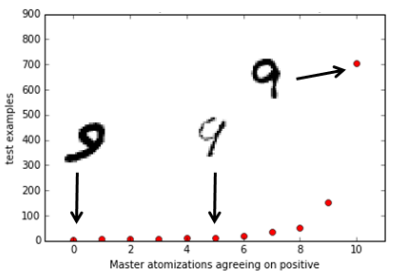
\includegraphics[scale=0.5]{fig/hand.png}
            \label{fig:hand}
        \end{figure}}
        \item<2-> N-rainhas
        \only<2>{\begin{figure}
            \centering
            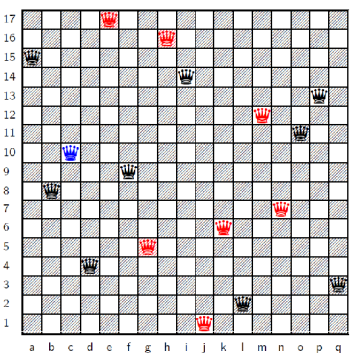
\includegraphics[scale=0.5]{fig/nrainhas.png}
            \label{fig:nrainhas}
        \end{figure}}
    \end{itemize}
\end{frame}

\section{Definições}
\subsection*{Elementos da Álgebra}
\begin{frame}{\subsecname}
    \uncover<1->{Álgebra: $M = \mathbf{T}(M)~\dot\cup~ \mathbf{C}(M)~\dot\cup~\mathbf{A}(M)$}
\begin{itemize}
    \item<2-> Termos $\mathbf{T}(M)$\\\vspace{2 mm}
    \allTerms
    \item<3-> Constantes $\mathbf{C}(M)$ \\\vspace{2 mm}
    \allConstants
    \item<4-> Átomos $\mathbf{A}(M)$
    \begin{itemize}
        \item<4-> Unidades de aprendizagem criadas pelo algoritmo
        \item<5-> Representados em geral por letras gregas ($\phi$, $\epsilon$, $\zeta$,...)
    \end{itemize}
\end{itemize}
\end{frame}
\subsection*{A operação combinar}
\begin{frame}
    \frametitle{\subsecname}
    \uncover<1->{$\odot\colon M\times M\to M$}
    \begin{itemize}
        \item<2-> Axiomas
        \begin{itemize}
            \item<2-> Idempotência\\
                \quad $a \odot a = a$
            \item<3-> Comutatividade\\
                \quad $a \odot b = b \odot a$
            \item<4-> Associatividade\\
                \quad $a \odot (b \odot c) = (a \odot b) \odot c$
        \end{itemize}
        \item<5-> Exemplo\\\vspace{2 mm}
        {\renewcommand*{\TermScale}{0.4}
    $
        \vcenter{\hbox{\BBWW}}
        =
        \vcenter{\hbox{\constant{1/3/black}}}
        \odot
        \vcenter{\hbox{\constant{1/1/black}}}
        \odot
        \vcenter{\hbox{\constant{3/1/white}}}
        \odot
        \vcenter{\hbox{\constant{3/3/white}}}
    $}
    \end{itemize}
\end{frame}

\section{O Algoritmo}
\subsection{\texorpdfstring{A Álgebra Principal $M$}{A Álgebra Principal M}}
\begin{frame}{\subsecname}
\renewcommand*{\TermScale}{0.4}
\centering
\begin{tikzpicture}[
every node/.style = {
    % shape=circle,
    % draw,
    align=center,
    minimum size=22pt,
    inner sep=0pt,
    outer sep=0pt,
},
term/.append style = {
    uncover={<1,4->},
},
constant/.append style = {
    uncover={<2,4->},
},
atom/.append style = {
    uncover={<3,4->},
},
]]
%
\node[atom, shape = circle, draw] (zero) at (0,0) {\zeroslash};
\coordinate[at=(zero.north)] (azero);
\coordinate[at=(zero.west)] (lzero);
\newcommand*{\sep}{0.9}
\foreach \x in {1, 2, 3, 4, 5, 6, 7, 8}{
  \node[constant] (c\x) at (\x*\sep - 4*\sep, 2) {\const{\x}};
  \coordinate[below=0.1cm,at=(c\x.south)] (bc\x);
  \coordinate[above=0.1cm,at=(c\x.north)] (ac\x);
}
\node[constant, shape = circle, draw] (v) at (-4.5*\sep,2) {$v$};
\coordinate[below=0.1cm,at=(v.south)] (bv);
\foreach \x in {1, 2, 3, 4, 5, 6, 7, 8}{
  \draw[uncover={<13->}] (azero) -- (bc\x);
}
\draw[uncover={<13->}] (azero) -- (bv);
%
\renewcommand*{\TermScale}{0.6}
\renewcommand*{\sep}{1.4}
\foreach \x in {1, 2}{
  \node[term] (T\x) at (\x*\sep - 2.5*\sep - 0.1, 5) {\Term{\x}};
  \coordinate[below=0.1cm,at=(T\x.south)] (bT\x);
}
\draw[term, very thick] (-0.5*\sep + 0.5*\sep, 5 - \TermScale) -- (-0.5*\sep + 0.5*\sep, 5 + \TermScale);
\foreach \x in {3, 4, 5}{
  \node[term] (T\x) at (\x*\sep - 2.5*\sep + 0.1, 5) {\Term{\x}};
  \coordinate[below=0.1cm,at=(T\x.south)] (bT\x);
}
%
\foreach \x in {1, 2, 7, 8}{\draw[uncover={<7,12->}] (ac\x) -- (bT1);}
\foreach \x in {5, 6, 3, 4}{\draw[uncover={<8,12->}] (ac\x) -- (bT2);}
\foreach \x in {5, 2, 7, 4}{\draw[uncover={<9,12->}] (ac\x) -- (bT3);}
\foreach \x in {5, 6, 3, 8}{\draw[uncover={<10,12->}] (ac\x) -- (bT4);}
\foreach \x in {5, 6, 7, 4}{\draw[uncover={<11,12->}] (ac\x) -- (bT5);}
%
\foreach \x in {1, 2, 3, 4, 5}{
    \draw[uncover={<14->}, blue] (azero) -- (bT\x);
}
\node[visible on={<5>}, below=1cm,at=(v.south)] (text_v) {constante alvo};
\draw[visible on={<5>}, -{stealth}] (text_v) -- (bv);
\node[visible on={<6>}, left=1cm,at=(zero.west), inner sep=0.1cm] (text_0) {átomo zero};
\draw[visible on={<6>}, -{stealth}] (text_0) -- (lzero);

\end{tikzpicture}
\end{frame}
\subsection{\texorpdfstring{A Álgebra Dual $M^\star$}{A Álgebra Principal M*}}
\newcommand*{\dualcolor}{blue}
\newcommand*{\dual}[1]{{\color{\dualcolor}[}#1{\color{\dualcolor}]}}
\begin{frame}{\subsecname}
\centering
\scalebox{0.5}{
\begin{tikzpicture}[
every node/.style = {
    % shape=circle,
    % draw,
    align=center,
    minimum size=22pt,
    inner sep=0pt,
    outer sep=0pt,
},
]]
%
\node[shape = circle, draw] (zero) at (0,0) {\zeroslash};
\coordinate[at=(zero.north)] (azero);
\coordinate[at=(zero.west)] (lzero);
\newcommand*{\sep}{1.1}
\foreach \x in {1, 2, 3, 4, 5, 6, 7, 8}{
  \node[] (c\x) at (\x*\sep - 4*\sep, 2) {\const{\x}};
  \coordinate[below=0.1cm,at=(c\x.south)] (bc\x);
  \coordinate[above=0.1cm,at=(c\x.north)] (ac\x);
}
\node[shape = circle, draw] (v) at (-4.5*\sep,2) {$v$};
\coordinate[below=0.1cm,at=(v.south)] (bv);
\foreach \x in {1, 2, 3, 4, 5, 6, 7, 8}{
  \draw[] (azero) -- (bc\x);
}
\draw[] (azero) -- (bv);
%
\renewcommand*{\TermScale}{0.6}
\renewcommand*{\sep}{1.4}
\foreach \x in {1, 2}{
  \node[] (T\x) at (\x*\sep - 2.5*\sep - 0.1, 5) {\Term{\x}};
  \coordinate[below=0.1cm,at=(T\x.south)] (bT\x);
}
\draw[very thick] (-0.5*\sep + 0.5*\sep, 5 - \TermScale) -- (-0.5*\sep + 0.5*\sep, 5 + \TermScale);
\foreach \x in {3, 4, 5}{
  \node[] (T\x) at (\x*\sep - 2.5*\sep + 0.1, 5) {\Term{\x}};
  \coordinate[below=0.1cm,at=(T\x.south)] (bT\x);
}
%
\foreach \x in {1, 2, 7, 8}{\draw[] (ac\x) -- (bT1);}
\foreach \x in {5, 6, 3, 4}{\draw[] (ac\x) -- (bT2);}
\foreach \x in {5, 2, 7, 4}{\draw[] (ac\x) -- (bT3);}
\foreach \x in {5, 6, 3, 8}{\draw[] (ac\x) -- (bT4);}
\foreach \x in {5, 6, 7, 4}{\draw[] (ac\x) -- (bT5);}
%
\end{tikzpicture}
\quad
\begin{tikzpicture}[
every node/.style = {
    % shape=circle,
    % draw,
    align=center,
    minimum size=22pt,
    inner sep=0pt,
    outer sep=0pt,
},
dual/.style = {
    color = \dualcolor,
},
]]
%
\node[shape = circle, draw] (zero) at (0,0) {\dual{\zeroslash}};
\coordinate[at=(zero.south)] (bzero);
\newcommand*{\sep}{1.1}
\foreach \x in {1, 2, 3, 4, 5, 6, 7, 8}{
  \node[dual] (c\x) at (\x*\sep - 4*\sep, -2) {\const{\x}};
  \coordinate[below=0.1cm,at=(c\x.south)] (bc\x);
  \coordinate[above=0.1cm,at=(c\x.north)] (ac\x);
}
\node[shape = circle, draw] (v) at (-4.5*\sep,-2) {\dual{$v$}};
\coordinate[above=0.1cm,at=(v.north)] (av);
\coordinate[below=0.1cm,at=(v.south)] (bv);
\foreach \x in {1, 2, 3, 4, 5, 6, 7, 8}{
  \draw[] (bzero) -- (ac\x);
}
\draw[] (bzero) -- (av);
%
\renewcommand*{\TermScale}{0.6}
\renewcommand*{\sep}{1.4}
\foreach \x in {1, 2}{
  \node[dual] (T\x) at (\x*\sep - 2.5*\sep - 0.1, -5) {\Term{\x}};
  \coordinate[above=0.1cm,at=(T\x.north)] (aT\x);
  \coordinate[below=0.1cm,at=(T\x.south)] (bT\x);
}
\draw[very thick] (-0.5*\sep + 0.5*\sep, -5 + \TermScale) -- (-0.5*\sep + 0.5*\sep, -5 - \TermScale);
\foreach \x in {3, 4, 5}{
  \node[dual] (T\x) at (\x*\sep - 2.5*\sep + 0.1, -5) {\Term{\x}};
  \coordinate[above=0.1cm,at=(T\x.north)] (aT\x);
  \coordinate[below=0.1cm,at=(T\x.south)] (bT\x);
}
%
\foreach \x in {1, 2, 7, 8}{\draw[] (bc\x) -- (aT1);}
\foreach \x in {5, 6, 3, 4}{\draw[] (bc\x) -- (aT2);}
\foreach \x in {5, 2, 7, 4}{\draw[] (bc\x) -- (aT3);}
\foreach \x in {5, 6, 3, 8}{\draw[] (bc\x) -- (aT4);}
\foreach \x in {5, 6, 7, 4}{\draw[] (bc\x) -- (aT5);}
%
\end{tikzpicture}
}
\end{frame}
%
\begin{frame}{\subsecname}
\centering   
\begin{tikzpicture}[
every node/.style = {
    % shape=circle,
    % draw,
    align=center,
    minimum size=22pt,
    inner sep=0pt,
    outer sep=0pt,
},
dual/.style = {
    color = \dualcolor,
},
]]
%
\node[shape = circle, draw] (zero) at (0,0) {\dual{\zeroslash}};
\coordinate[at=(zero.south)] (bzero);
\newcommand*{\sep}{1.1}
\foreach \x in {1, 2, 3, 4, 5, 6, 7, 8}{
  \node[dual] (c\x) at (\x*\sep - 4*\sep, -2) {\const{\x}};
  \coordinate[below=0.1cm,at=(c\x.south)] (bc\x);
  \coordinate[above=0.1cm,at=(c\x.north)] (ac\x);
}
\node[shape = circle, draw] (v) at (-4.5*\sep,-2) {\dual{$v$}};
\coordinate[above=0.1cm,at=(v.north)] (av);
\coordinate[below=0.1cm,at=(v.south)] (bv);
\foreach \x in {1, 2, 3, 4, 5, 6, 7, 8}{
  \draw[] (bzero) -- (ac\x);
}
\draw[] (bzero) -- (av);
%
\renewcommand*{\TermScale}{0.6}
\renewcommand*{\sep}{1.4}
\foreach \x in {1, 2}{
  \node[dual] (T\x) at (\x*\sep - 2.5*\sep - 0.1, -5) {\Term{\x}};
  \coordinate[above=0.1cm,at=(T\x.north)] (aT\x);
  \coordinate[below=0.1cm,at=(T\x.south)] (bT\x);
}
\draw[very thick] (-0.5*\sep + 0.5*\sep, -5 + \TermScale) -- (-0.5*\sep + 0.5*\sep, -5 - \TermScale);
\foreach \x in {3, 4, 5}{
  \node[dual] (T\x) at (\x*\sep - 2.5*\sep + 0.1, -5) {\Term{\x}};
  \coordinate[above=0.1cm,at=(T\x.north)] (aT\x);
  \coordinate[below=0.1cm,at=(T\x.south)] (bT\x);
}
%
\foreach \x in {1, 2, 7, 8}{\draw[] (bc\x) -- (aT1);}
\foreach \x in {5, 6, 3, 4}{\draw[] (bc\x) -- (aT2);}
\foreach \x in {5, 2, 7, 4}{\draw[] (bc\x) -- (aT3);}
\foreach \x in {5, 6, 3, 8}{\draw[] (bc\x) -- (aT4);}
\foreach \x in {5, 6, 7, 4}{\draw[] (bc\x) -- (aT5);}
%
\node[uncover={<3->}, shape=circle, draw] (zero_star) at (0, -7) {\zeroslash$^{\star}$};
\coordinate[at=(zero_star.north)] (azero_star);
\foreach \x in {1, 2, 3, 4, 5}{
  \draw[uncover={<3->}] (azero_star) -- (bT\x);
}
\foreach \x in {1, 2}{
    \draw[uncover={<2->}] (bv) -- (aT\x);
}
\end{tikzpicture}
\end{frame}
\subsection{Modelos Atomizados}
\begin{frame}{\subsecname}
    \begin{itemize}
        \item Definições: \\
            \uncover<1-> {\[a < b \iff \mathbf{GL^a}(a) \subset \mathbf{GL^a}(b)\]}\\
            \uncover<2->{\[\mathbf{GL^a}(a) = \{\phi\in\mathbf{A}(M)\colon\phi\to a\}\]}
        \item<3-> Objetivo: \\
            \[\forall T_i^{+} \in R^{+}\colon v < T_i^{+} \iff \mathbf{GL^a}(v) \subset \mathbf{GL^a}(T_i^{+})\]
            \[\forall T_i^{-} \in R^{-}\colon v \not< T_i^{-} \iff \mathbf{GL^a}(v) \subset \mathbf{GL^a}(T_i^{-})\]
    \end{itemize}
\end{frame}
\subsection{Traço e Restrições}
\begin{frame}{Traço}
\begin{itemize}
    \item<1-> Definição de traço:
        \[\mathbf{Tr}(x) \equiv \cap_{\phi \in \mathbf{GL^a}(x)} \mathbf{GL^{a}}([\phi]) \]
    \item<2-> Linearidade:
        \[\mathbf{Tr}(a \odot b) = \mathbf{Tr}(a) \cap \mathbf{Tr}(b)\]
    \item<3-> Restrição:
        \[ a < b \implies \mathbf{Tr}(b) \subset \mathbf{Tr}(a)\]
\end{itemize}
\end{frame}
\begin{frame}{Restrições de Traço}
\[ a < b \implies \mathbf{Tr}(b) \subset \mathbf{Tr}(a)\]
\begin{itemize}
    \item<1-> $\mathrm{for}~v < T_i^+~\mathrm{enforce}~
    \mathbf{Tr}(T_i^+) \subset \mathbf{Tr}(v) $
    \item<2-> $\mathrm{for}~v \not< T_i^-~\mathrm{enforce}~
    \mathbf{Tr}(T_i^-) \not\subset \mathbf{Tr}(v) $
\end{itemize}
\end{frame}
\begin{frame}{Traço e Restrições}
\centering
    \begin{tikzpicture}[
every node/.style = {
    % shape=circle,
    % draw,
    align=center,
    minimum size=22pt,
    inner sep=0pt,
    outer sep=0pt,
},
dual/.style = {
    color = \dualcolor,
},
]]
%
\node[shape = circle, draw] (zero) at (0,0) {\dual{\zeroslash}};
\coordinate[at=(zero.south)] (bzero);
\newcommand*{\sep}{1.1}
\foreach \x in {1, 2, 3, 4, 5, 6, 7, 8}{
  \node[dual] (c\x) at (\x*\sep - 4*\sep, -2) {\const{\x}};
  \coordinate[below=0.1cm,at=(c\x.south)] (bc\x);
  \coordinate[above=0.1cm,at=(c\x.north)] (ac\x);
}
\node[shape = circle, draw] (v) at (-4.5*\sep,-2) {\dual{$v$}};
\coordinate[above=0.1cm,at=(v.north)] (av);
\coordinate[below=0.1cm,at=(v.south)] (bv);
\foreach \x in {1, 2, 3, 4, 5, 6, 7, 8}{
  \draw[] (bzero) -- (ac\x);
}
\draw[] (bzero) -- (av);
%
\renewcommand*{\TermScale}{0.6}
\renewcommand*{\sep}{1.4}
\foreach \x in {1, 2}{
  \node[dual] (T\x) at (\x*\sep - 2.5*\sep - 0.1, -5) {\Term{\x}};
  \coordinate[above=0.1cm,at=(T\x.north)] (aT\x);
  \coordinate[below=0.1cm,at=(T\x.south)] (bT\x);
}
\draw[very thick] (-0.5*\sep + 0.5*\sep, -5 + \TermScale) -- (-0.5*\sep + 0.5*\sep, -5 - \TermScale);
\foreach \x in {3, 4, 5}{
  \node[dual] (T\x) at (\x*\sep - 2.5*\sep + 0.1, -5) {\Term{\x}};
  \coordinate[above=0.1cm,at=(T\x.north)] (aT\x);
  \coordinate[below=0.1cm,at=(T\x.south)] (bT\x);
}
%
\foreach \x in {1, 2, 7, 8}{\draw[] (bc\x) -- (aT1);}
\foreach \x in {5, 6, 3, 4}{\draw[] (bc\x) -- (aT2);}
\foreach \x in {5, 2, 7, 4}{\draw[] (bc\x) -- (aT3);}
\foreach \x in {5, 6, 3, 8}{\draw[] (bc\x) -- (aT4);}
\foreach \x in {5, 6, 7, 4}{\draw[] (bc\x) -- (aT5);}
%
\node[shape=circle, draw] (zero_star) at (-1.5*\sep - 0.1, -7) {\zeroslash$^{\star}$};
\coordinate[at=(zero_star.north)] (azero_star);
\foreach \x in {1, 2, 3, 4, 5}{
  \draw[] (azero_star) -- (bT\x);
}
\foreach \x in {1, 2}{
    \draw[] (bv) -- (aT\x);
}
\foreach \x in {1, 2, 3}{
    \node[uncover={<2->}, shape = circle, draw] (zeta\x) at (\x*\sep - 0.5*\sep+ 0.1, -7) {$\zeta_\x$};
    \coordinate[above=0.1cm,at=(zeta\x.north)] (azeta\x);
}
\draw[uncover={<2->}] (azeta1) -- (bT3);
\draw[uncover={<2->}] (azeta2) -- (bT4);
\draw[uncover={<2->}] (azeta3) -- (bT5);
\end{tikzpicture}
\end{frame}
\begin{frame}{Traço e Restrições}
\centering
    \scalebox{0.5}{
\begin{tikzpicture}[
every node/.style = {
    % shape=circle,
    % draw,
    align=center,
    minimum size=22pt,
    inner sep=0pt,
    outer sep=0pt,
},
]]
%
\node[shape = circle, draw] (zero) at (1.1,0) {\zeroslash};
\coordinate[at=(zero.north)] (azero);
\coordinate[at=(zero.west)] (lzero);
\newcommand*{\sep}{1.1}
\foreach \x in {1, 2, 3, 4, 5, 6, 7, 8}{
  \node[] (c\x) at (\x*\sep - 4*\sep, 2) {\const{\x}};
  \coordinate[below=0.1cm,at=(c\x.south)] (bc\x);
  \coordinate[above=0.1cm,at=(c\x.north)] (ac\x);
}
\node[shape = circle, draw] (v) at (-4.5*\sep,2) {$v$};
\coordinate[below=0.1cm,at=(v.south)] (bv);
\foreach \x in {1, 2, 3, 4, 5, 6, 7, 8}{
  \draw[] (azero) -- (bc\x);
}
\draw[] (azero) -- (bv);
%
\renewcommand*{\TermScale}{0.6}
\renewcommand*{\sep}{1.4}
\foreach \x in {1, 2}{
  \node[] (T\x) at (\x*\sep - 2.5*\sep - 0.1, 5) {\Term{\x}};
  \coordinate[below=0.1cm,at=(T\x.south)] (bT\x);
}
\draw[very thick] (-0.5*\sep + 0.5*\sep, 5 - \TermScale) -- (-0.5*\sep + 0.5*\sep, 5 + \TermScale);
\foreach \x in {3, 4, 5}{
  \node[] (T\x) at (\x*\sep - 2.5*\sep + 0.1, 5) {\Term{\x}};
  \coordinate[below=0.1cm,at=(T\x.south)] (bT\x);
}
%
\foreach \x in {1, 2, 7, 8}{\draw[] (ac\x) -- (bT1);}
\foreach \x in {5, 6, 3, 4}{\draw[] (ac\x) -- (bT2);}
\foreach \x in {5, 2, 7, 4}{\draw[] (ac\x) -- (bT3);}
\foreach \x in {5, 6, 3, 8}{\draw[] (ac\x) -- (bT4);}
\foreach \x in {5, 6, 7, 4}{\draw[] (ac\x) -- (bT5);}
%
\node[uncover={<2->}, shape = circle, draw] (phi) at (-4.5*1.1, 0) {$\phi$};
\coordinate[at=(phi.north)] (aphi);
\draw[uncover={<2->}] (aphi) -- (bv);
%
%
\renewcommand*{\sep}{1.1}
\node[uncover={<3->}, shape = circle, draw] (epsilon1) at (-3*\sep, 0) {$\epsilon_1$};
\coordinate[above=0.1cm,at=(epsilon1.north)] (aepsilon1);
\node[uncover={<3->}, shape = circle, draw] (epsilon2) at (-1*\sep, 0) {$\epsilon_2$};
\coordinate[above=0.1cm,at=(epsilon2.north)] (aepsilon2);
\node[uncover={<3->}, shape = circle, draw] (epsilon3) at (0*\sep, 0) {$\epsilon_3$};
\coordinate[above=0.1cm,at=(epsilon3.north)] (aepsilon3);
\draw[uncover={<3->}] (bc1) -- (aepsilon1);
\draw[uncover={<3->}] (bc3) -- (aepsilon2);
\draw[uncover={<3->}] (bc4) -- (aepsilon3);
\end{tikzpicture}
\quad
%
%
%
%
%
%
\begin{tikzpicture}[
every node/.style = {
    % shape=circle,
    % draw,
    align=center,
    minimum size=22pt,
    inner sep=0pt,
    outer sep=0pt,
},
dual/.style = {
    color = \dualcolor,
},
]]
%
\node[shape = circle, draw] (zero) at (1.1,0) {\dual{\zeroslash}};
\coordinate[at=(zero.south)] (bzero);
\newcommand*{\sep}{1.1}
\foreach \x in {1, 2, 3, 4, 5, 6, 7, 8}{
  \node[dual] (c\x) at (\x*\sep - 4*\sep, -2) {\const{\x}};
  \coordinate[below=0.1cm,at=(c\x.south)] (bc\x);
  \coordinate[above=0.1cm,at=(c\x.north)] (ac\x);
}
\node[shape = circle, draw] (v) at (-4.5*\sep,-2) {\dual{$v$}};
\coordinate[above=0.1cm,at=(v.north)] (av);
\coordinate[below=0.1cm,at=(v.south)] (bv);
\foreach \x in {1, 2, 3, 4, 5, 6, 7, 8}{
  \draw[] (bzero) -- (ac\x);
}
\draw[] (bzero) -- (av);
%
\renewcommand*{\TermScale}{0.6}
\renewcommand*{\sep}{1.4}
\foreach \x in {1, 2}{
  \node[dual] (T\x) at (\x*\sep - 2.5*\sep - 0.1, -5) {\Term{\x}};
  \coordinate[above=0.1cm,at=(T\x.north)] (aT\x);
  \coordinate[below=0.1cm,at=(T\x.south)] (bT\x);
}
\draw[very thick] (-0.5*\sep + 0.5*\sep, -5 + \TermScale) -- (-0.5*\sep + 0.5*\sep, -5 - \TermScale);
\foreach \x in {3, 4, 5}{
  \node[dual] (T\x) at (\x*\sep - 2.5*\sep + 0.1, -5) {\Term{\x}};
  \coordinate[above=0.1cm,at=(T\x.north)] (aT\x);
  \coordinate[below=0.1cm,at=(T\x.south)] (bT\x);
}
%
\foreach \x in {1, 2, 7, 8}{\draw[] (bc\x) -- (aT1);}
\foreach \x in {5, 6, 3, 4}{\draw[] (bc\x) -- (aT2);}
\foreach \x in {5, 2, 7, 4}{\draw[] (bc\x) -- (aT3);}
\foreach \x in {5, 6, 3, 8}{\draw[] (bc\x) -- (aT4);}
\foreach \x in {5, 6, 7, 4}{\draw[] (bc\x) -- (aT5);}
%
\node[shape=circle, draw] (zero_star) at (-1.5*\sep - 0.1, -7) {\zeroslash$^{\star}$};
\coordinate[at=(zero_star.north)] (azero_star);
\foreach \x in {1, 2, 3, 4, 5}{
  \draw[] (azero_star) -- (bT\x);
}
\foreach \x in {1, 2}{
    \draw[] (bv) -- (aT\x);
}
\foreach \x in {1, 2, 3}{
    \node[shape = circle, draw] (zeta\x) at (\x*\sep - 0.5*\sep+ 0.1, -7) {$\zeta_\x$};
    \coordinate[above=0.1cm,at=(zeta\x.north)] (azeta\x);
}
\draw[] (azeta1) -- (bT3);
\draw[] (azeta2) -- (bT4);
\draw[] (azeta3) -- (bT5);

\node[uncover={<2->}, shape = circle, draw] (phi) at (-4.5*1.1, 0) {\dual{$\phi$}};
\coordinate[at=(phi.south)] (bphi);
\draw[uncover={<2->}] (bphi) -- (av);

\renewcommand*{\sep}{1.1}
\node[uncover={<3->}, shape = circle, draw] (epsilon1) at (-3*\sep, 0) {\dual{$\epsilon_1$}};
\coordinate[above=0.1cm,at=(epsilon1.south)] (bepsilon1);
\node[uncover={<3->}, shape = circle, draw] (epsilon2) at (-1*\sep, 0) {\dual{$\epsilon_2$}};
\coordinate[above=0.1cm,at=(epsilon2.south)] (bepsilon2);
\node[uncover={<3->}, shape = circle, draw] (epsilon3) at (0*\sep, 0) {\dual{$\epsilon_3$}};
\coordinate[above=0.1cm,at=(epsilon3.south)] (bepsilon3);
\draw[uncover={<3->}] (ac1) -- (bepsilon1);
\draw[uncover={<3->}] (ac3) -- (bepsilon2);
\draw[uncover={<3->}] (ac4) -- (bepsilon3);

\end{tikzpicture}
}
\end{frame}
\subsection{Cruzamento}
\begin{frame}{\subsecname}
\centering
    \scalebox{0.5}{
\begin{tikzpicture}[
every node/.style = {
    % shape=circle,
    % draw,
    align=center,
    minimum size=22pt,
    inner sep=0pt,
    outer sep=0pt,
},
]]
%
\node[shape = circle, draw] (zero) at (1.1,0) {\zeroslash};
\coordinate[at=(zero.north)] (azero);
\coordinate[at=(zero.west)] (lzero);
\newcommand*{\sep}{1.1}
\foreach \x in {1, 2, 3, 4, 5, 6, 7, 8}{
  \node[] (c\x) at (\x*\sep - 4*\sep, 2) {\const{\x}};
  \coordinate[below=0.1cm,at=(c\x.south)] (bc\x);
  \coordinate[above=0.1cm,at=(c\x.north)] (ac\x);
}
\node[shape = circle, draw] (v) at (-4.5*\sep,2) {$v$};
\coordinate[below=0.1cm,at=(v.south)] (bv);
\foreach \x in {1, 2, 3, 4, 5, 6, 7, 8}{
  \draw[] (azero) -- (bc\x);
}
\draw[] (azero) -- (bv);
%
\renewcommand*{\TermScale}{0.6}
\renewcommand*{\sep}{1.4}
\foreach \x in {1, 2}{
  \node[] (T\x) at (\x*\sep - 2.5*\sep - 0.1, 5) {\Term{\x}};
  \coordinate[below=0.1cm,at=(T\x.south)] (bT\x);
}
\draw[very thick] (-0.5*\sep + 0.5*\sep, 5 - \TermScale) -- (-0.5*\sep + 0.5*\sep, 5 + \TermScale);
\foreach \x in {3, 4, 5}{
  \node[] (T\x) at (\x*\sep - 2.5*\sep + 0.1, 5) {\Term{\x}};
  \coordinate[below=0.1cm,at=(T\x.south)] (bT\x);
}
%
\foreach \x in {1, 2, 7, 8}{\draw[] (ac\x) -- (bT1);}
\foreach \x in {5, 6, 3, 4}{\draw[] (ac\x) -- (bT2);}
\foreach \x in {5, 2, 7, 4}{\draw[] (ac\x) -- (bT3);}
\foreach \x in {5, 6, 3, 8}{\draw[] (ac\x) -- (bT4);}
\foreach \x in {5, 6, 7, 4}{\draw[] (ac\x) -- (bT5);}
%
\node[shape = circle, draw] (phi) at (-4.5*1.1, 0) {$\phi$};
\coordinate[at=(phi.north)] (aphi);
\draw[] (aphi) -- (bv);
%
%
\renewcommand*{\sep}{1.1}
\node[shape = circle, draw] (epsilon1) at (-3*\sep, 0) {$\epsilon_1$};
\coordinate[at=(epsilon1.north)] (aepsilon1);
\node[shape = circle, draw] (epsilon2) at (-1*\sep, 0) {$\epsilon_2$};
\coordinate[at=(epsilon2.north)] (aepsilon2);
\node[shape = circle, draw] (epsilon3) at (0*\sep, 0) {$\epsilon_3$};
\coordinate[at=(epsilon3.north)] (aepsilon3);
\draw (bc1) -- (aepsilon1);
\draw (bc3) -- (aepsilon2);
\draw (bc4) -- (aepsilon3);
%
%
\node[uncover={<2->}, shape = circle, draw] (phi1) at (-4.5*1.1*0.5 -3*\sep*0.5, -1) {$\phi_1$};
\coordinate[at=(phi.south)] (bphi);

\coordinate[at=(phi1.north)] (aphi1);
\coordinate[at=(epsilon1.south)] (bepsilon1);
\draw[uncover={<2->}] (aphi1) -- (bphi);
\draw[uncover={<2->}] (aphi1) -- (bepsilon1);
\end{tikzpicture}
\quad
%
%
%
%
%
%
\begin{tikzpicture}[
every node/.style = {
    % shape=circle,
    % draw,
    align=center,
    minimum size=22pt,
    inner sep=0pt,
    outer sep=0pt,
},
dual/.style = {
    color = \dualcolor,
},
]]
%
\node[shape = circle, draw] (zero) at (1.1,0) {\dual{\zeroslash}};
\coordinate[at=(zero.south)] (bzero);
\newcommand*{\sep}{1.1}
\foreach \x in {1, 2, 3, 4, 5, 6, 7, 8}{
  \node[dual] (c\x) at (\x*\sep - 4*\sep, -2) {\const{\x}};
  \coordinate[below=0.1cm,at=(c\x.south)] (bc\x);
  \coordinate[above=0.1cm,at=(c\x.north)] (ac\x);
}
\node[shape = circle, draw] (v) at (-4.5*\sep,-2) {\dual{$v$}};
\coordinate[above=0.1cm,at=(v.north)] (av);
\coordinate[below=0.1cm,at=(v.south)] (bv);
\foreach \x in {1, 2, 3, 4, 5, 6, 7, 8}{
  \draw[] (bzero) -- (ac\x);
}
\draw[] (bzero) -- (av);
%
\renewcommand*{\TermScale}{0.6}
\renewcommand*{\sep}{1.4}
\foreach \x in {1, 2}{
  \node[dual] (T\x) at (\x*\sep - 2.5*\sep - 0.1, -5) {\Term{\x}};
  \coordinate[above=0.1cm,at=(T\x.north)] (aT\x);
  \coordinate[below=0.1cm,at=(T\x.south)] (bT\x);
}
\draw[very thick] (-0.5*\sep + 0.5*\sep, -5 + \TermScale) -- (-0.5*\sep + 0.5*\sep, -5 - \TermScale);
\foreach \x in {3, 4, 5}{
  \node[dual] (T\x) at (\x*\sep - 2.5*\sep + 0.1, -5) {\Term{\x}};
  \coordinate[above=0.1cm,at=(T\x.north)] (aT\x);
  \coordinate[below=0.1cm,at=(T\x.south)] (bT\x);
}
%
\foreach \x in {1, 2, 7, 8}{\draw[] (bc\x) -- (aT1);}
\foreach \x in {5, 6, 3, 4}{\draw[] (bc\x) -- (aT2);}
\foreach \x in {5, 2, 7, 4}{\draw[] (bc\x) -- (aT3);}
\foreach \x in {5, 6, 3, 8}{\draw[] (bc\x) -- (aT4);}
\foreach \x in {5, 6, 7, 4}{\draw[] (bc\x) -- (aT5);}
%
\node[shape=circle, draw] (zero_star) at (-1.5*\sep - 0.1, -7) {\zeroslash$^{\star}$};
\coordinate[at=(zero_star.north)] (azero_star);
\foreach \x in {1, 2, 3, 4, 5}{
  \draw[] (azero_star) -- (bT\x);
}
\foreach \x in {1, 2}{
    \draw[] (bv) -- (aT\x);
}
\foreach \x in {1, 2, 3}{
    \node[shape = circle, draw] (zeta\x) at (\x*\sep - 0.5*\sep+ 0.1, -7) {$\zeta_\x$};
    \coordinate[above=0.1cm,at=(zeta\x.north)] (azeta\x);
}
\draw[] (azeta1) -- (bT3);
\draw[] (azeta2) -- (bT4);
\draw[] (azeta3) -- (bT5);

\node[shape = circle, draw] (phi) at (-4.5*1.1, 0) {\dual{$\phi$}};
\coordinate[at=(phi.south)] (bphi);
\draw[] (bphi) -- (av);

\renewcommand*{\sep}{1.1}
\node[shape = circle, draw] (epsilon1) at (-3*\sep, 0) {\dual{$\epsilon_1$}};
\coordinate[at=(epsilon1.south)] (bepsilon1);
\node[shape = circle, draw] (epsilon2) at (-1*\sep, 0) {\dual{$\epsilon_2$}};
\coordinate[at=(epsilon2.south)] (bepsilon2);
\node[shape = circle, draw] (epsilon3) at (0*\sep, 0) {\dual{$\epsilon_3$}};
\coordinate[at=(epsilon3.south)] (bepsilon3);
\draw[] (ac1) -- (bepsilon1);
\draw[] (ac3) -- (bepsilon2);
\draw[] (ac4) -- (bepsilon3);
%
%
\node[uncover={<2->}, shape = circle, draw] (phi1) at (-4.5*1.1*0.5 -3*\sep*0.5, +1) {\dual{$\phi_1$}};
\coordinate[at=(phi.north)] (aphi);

\coordinate[at=(phi1.south)] (bphi1);
\coordinate[at=(epsilon1.north)] (aepsilon1);
\draw[uncover={<2->}] (bphi1) -- (aphi);
\draw[uncover={<2->}] (bphi1) -- (aepsilon1);
\end{tikzpicture}
}
\end{frame}
\begin{frame}{\subsecname}
\centering
    \scalebox{0.5}{
\begin{tikzpicture}[
every node/.style = {
    % shape=circle,
    % draw,
    align=center,
    minimum size=22pt,
    inner sep=0pt,
    outer sep=0pt,
},
]]
%
\node[shape = circle, draw] (zero) at (1.1,0) {\zeroslash};
\coordinate[at=(zero.north)] (azero);
\coordinate[at=(zero.west)] (lzero);
\newcommand*{\sep}{1.1}
\foreach \x in {1, 2, 3, 4, 5, 6, 7, 8}{
  \node[] (c\x) at (\x*\sep - 4*\sep, 2) {\const{\x}};
  \coordinate[below=0.1cm,at=(c\x.south)] (bc\x);
  \coordinate[above=0.1cm,at=(c\x.north)] (ac\x);
}
\node[shape = circle, draw] (v) at (-4.5*\sep,2) {$v$};
\coordinate[below=0.1cm,at=(v.south)] (bv);
\foreach \x in {1, 2, 3, 4, 5, 6, 7, 8}{
  \draw[] (azero) -- (bc\x);
}
\draw[] (azero) -- (bv);
%
\renewcommand*{\TermScale}{0.6}
\renewcommand*{\sep}{1.4}
\foreach \x in {1, 2}{
  \node[] (T\x) at (\x*\sep - 2.5*\sep - 0.1, 5) {\Term{\x}};
  \coordinate[below=0.1cm,at=(T\x.south)] (bT\x);
}
\draw[very thick] (-0.5*\sep + 0.5*\sep, 5 - \TermScale) -- (-0.5*\sep + 0.5*\sep, 5 + \TermScale);
\foreach \x in {3, 4, 5}{
  \node[] (T\x) at (\x*\sep - 2.5*\sep + 0.1, 5) {\Term{\x}};
  \coordinate[below=0.1cm,at=(T\x.south)] (bT\x);
}
%
\foreach \x in {1, 2, 7, 8}{\draw[] (ac\x) -- (bT1);}
\foreach \x in {5, 6, 3, 4}{\draw[] (ac\x) -- (bT2);}
\foreach \x in {5, 2, 7, 4}{\draw[] (ac\x) -- (bT3);}
\foreach \x in {5, 6, 3, 8}{\draw[] (ac\x) -- (bT4);}
\foreach \x in {5, 6, 7, 4}{\draw[] (ac\x) -- (bT5);}
%
\renewcommand*{\sep}{1.1}
\node[shape = circle, draw] (phi1) at (-4.5*1.1*0.5 -3*\sep*0.5, 0) {$\phi_1$};
\coordinate[at=(phi1.north)] (aphi1);
\node[shape = circle, draw] (epsilon2) at (-1*\sep, 0) {$\epsilon_2$};
\coordinate[at=(epsilon2.north)] (aepsilon2);
\node[shape = circle, draw] (epsilon3) at (0*\sep, 0) {$\epsilon_3$};
\coordinate[at=(epsilon3.north)] (aepsilon3);
\draw (bc1) -- (aphi1);
\draw (bv) -- (aphi1);
\draw (bc3) -- (aepsilon2);
\draw (bc4) -- (aepsilon3);
%
%
\end{tikzpicture}
\quad
%
%
%
%
%
%
\begin{tikzpicture}[
every node/.style = {
    % shape=circle,
    % draw,
    align=center,
    minimum size=22pt,
    inner sep=0pt,
    outer sep=0pt,
},
dual/.style = {
    color = \dualcolor,
},
]]
%
\node[shape = circle, draw] (zero) at (1.1,0) {\dual{\zeroslash}};
\coordinate[at=(zero.south)] (bzero);
\newcommand*{\sep}{1.1}
\foreach \x in {1, 2, 3, 4, 5, 6, 7, 8}{
  \node[dual] (c\x) at (\x*\sep - 4*\sep, -2) {\const{\x}};
  \coordinate[below=0.1cm,at=(c\x.south)] (bc\x);
  \coordinate[above=0.1cm,at=(c\x.north)] (ac\x);
}
\node[shape = circle, draw] (v) at (-4.5*\sep,-2) {\dual{$v$}};
\coordinate[above=0.1cm,at=(v.north)] (av);
\coordinate[below=0.1cm,at=(v.south)] (bv);
\foreach \x in {1, 2, 3, 4, 5, 6, 7, 8}{
  \draw[] (bzero) -- (ac\x);
}
\draw[] (bzero) -- (av);
%
\renewcommand*{\TermScale}{0.6}
\renewcommand*{\sep}{1.4}
\foreach \x in {1, 2}{
  \node[dual] (T\x) at (\x*\sep - 2.5*\sep - 0.1, -5) {\Term{\x}};
  \coordinate[above=0.1cm,at=(T\x.north)] (aT\x);
  \coordinate[below=0.1cm,at=(T\x.south)] (bT\x);
}
\draw[very thick] (-0.5*\sep + 0.5*\sep, -5 + \TermScale) -- (-0.5*\sep + 0.5*\sep, -5 - \TermScale);
\foreach \x in {3, 4, 5}{
  \node[dual] (T\x) at (\x*\sep - 2.5*\sep + 0.1, -5) {\Term{\x}};
  \coordinate[above=0.1cm,at=(T\x.north)] (aT\x);
  \coordinate[below=0.1cm,at=(T\x.south)] (bT\x);
}
%
\foreach \x in {1, 2, 7, 8}{\draw[] (bc\x) -- (aT1);}
\foreach \x in {5, 6, 3, 4}{\draw[] (bc\x) -- (aT2);}
\foreach \x in {5, 2, 7, 4}{\draw[] (bc\x) -- (aT3);}
\foreach \x in {5, 6, 3, 8}{\draw[] (bc\x) -- (aT4);}
\foreach \x in {5, 6, 7, 4}{\draw[] (bc\x) -- (aT5);}
%
\node[shape=circle, draw] (zero_star) at (-1.5*\sep - 0.1, -7) {\zeroslash$^{\star}$};
\coordinate[at=(zero_star.north)] (azero_star);
\foreach \x in {1, 2, 3, 4, 5}{
  \draw[] (azero_star) -- (bT\x);
}
\foreach \x in {1, 2}{
    \draw[] (bv) -- (aT\x);
}
\foreach \x in {1, 2, 3}{
    \node[shape = circle, draw] (zeta\x) at (\x*\sep - 0.5*\sep+ 0.1, -7) {$\zeta_\x$};
    \coordinate[above=0.1cm,at=(zeta\x.north)] (azeta\x);
}
\draw[] (azeta1) -- (bT3);
\draw[] (azeta2) -- (bT4);
\draw[] (azeta3) -- (bT5);

\renewcommand*{\sep}{1.1}
\node[shape = circle, draw] (phi1) at (-4.5*1.1*0.5 -3*\sep*0.5, 0) {\dual{$\phi_1$}};
\coordinate[at=(phi1.south)] (bphi1);
\node[shape = circle, draw] (epsilon2) at (-1*\sep, 0) {$\epsilon_2$};
\coordinate[at=(epsilon2.south)] (bepsilon2);
\node[shape = circle, draw] (epsilon3) at (0*\sep, 0) {$\epsilon_3$};
\coordinate[at=(epsilon3.south)] (bepsilon3);
\draw (ac1) -- (bphi1);
\draw (av) -- (bphi1);
\draw (ac3) -- (bepsilon2);
\draw (ac4) -- (bepsilon3);

\end{tikzpicture}
}
\end{frame}
\subsection{Redução de átomos}
\begin{frame}{\subsecname}
    Como no processo podem ser criados muitos átomos, existem rotinas que reduzem o número de átomos.
    \begin{itemize}
        \item As rotinas de redução são:
        \begin{itemize}
            \item Invariantes em relação ao traço das constantes.
            \item Estocásticas.
        \end{itemize}
        \item Há duas rotinas distintas:
        \begin{itemize}
            \item redução de $M$
            \item redução de $M^\star$
        \end{itemize}
    \end{itemize}
\end{frame}
\subsection{Treinamento em lote}
\begin{frame}{\subsecname}
    \begin{itemize}
        \item Termos e relações de fixação
        \item Economia de memória
    \end{itemize}
\end{frame}
\section*{Agradecimentos}
\begin{frame}{Obrigado por sua atenção!}
    \titlepage
\end{frame}
\end{document}
